\section{Ubhatob­yañ­janaka}

For the {\em ubhatob­yañ­janaka}\footnote{{\em Ubhato} meaning 'in both ways, on both sides' and {\em byañjana} or {\em vyañjana} means 'sign or mark'} we have less material to go on as for the {\em paṇḍaka}. It is only briefly mentioned in the Chinese Vinayas as those with two roots/faculties (二根) who are not allowed to ordain, but without any further explanation. The Therāvada Vinaya merely states that this person "acted and was acted upon". 

The commentarial literature is slightly more forthcoming but no less confusing as to the meaning of the word. The {\em Samantapāsādikā} identifies two types of {\em ubhatob­yañ­janaka} while the Chinese commentaries identify three. The {\em Samantapāsādikā}'s explanation is all the more puzzling because it describes the female {\em ubhatob­yañ­janaka} as having apparent female characteristics and the male characteristics hidden, but if they feel attracted to a women, they seem to be able to hide the female characteristic and make the male characteristic apparent. The opposite holds is described for a male {\em ubhatob­yañ­janaka}. Moreover the female {\em ubhatob­yañ­janaka} is able to become pregnant but also impregnate others so they become pregnant. This last aspect is also mentioned as one of the three types in the Chinese commentaries. The other two types in the Chinese are just described as being able to either get pregnant or impregnate others, just like females and males but with no further explanation as to why they are different from females and males. 

Apparently the ability to procreate is very important here and I would like to point out that it is humanly impossible to both conceive and impregnate\footnote{In \ref{appendix1}, \ref{hermaphrodite} I have described our current medical understanding of what it entails to both procreate as a male and a female}. However, as we have seen in the Vedic mythology this is a recurrent theme and there are many instances where a person is both mother and father. King Ila himself, in the form of the woman Ilā, becomes pregnant and bears a son. He/she is bound to keep on changing gender which also results in a change in sexual desires. In the {\em Mahābārata Anuśāsanaparvan}\footnote{MBh 13.12} we find the tale of King {\em Bhaṅgāśvana}, who is longing for a son, performs a divine ritual as a result of which he gets one hundred sons but in doing so invokes the anger of the god Indra, who turns him into a woman. As a woman she conceives another hundred sons.

Another story is recounted in the Buddhist {\em Dīrghāgama} Sutra T24 which describes how in the beginning all beings were male or female and were therefore subject to marriage. But the heavenly beings were bestowed with the gift to be free from marriage with no distinction between male and female; all became hermaphrodites (二根) with exactly the same faculties.

It seems therefore far more likely that our elusive {\em ubhatob­yañ­janaka} is nothing more than a mythological being and has no grounding in real life other than the embodiment of the feminine principle in the male. As with the {\em pakkhapaṇḍaka} ('half moon' {\em paṇḍaka}) it is not unthinkable that this was placed in the Vinaya to be complete, just under the section with the story of the mythological shape-shifting snake-turned-monk\footnote{In various Chinese texts other shape-shifting animals are mentioned too. F.i. T85 2792 毘尼心 0667c04–0667c05 mentions dragons, fox and deer}.

The other types of {\em ubhatob­yañ­janaka} mentioned in the commentaries seem to be similar in their ability to have sex as both a male and a female, but being impotent in one of these faculties. Again, this is not something we naturally find in human beings but is a theme extensively found in the Vedic myths\footnote{\cite{wendy} gives a particularly interesting account on androgyns in the ancient texts. These androgyns can have a large variety of possible characteristics and origins}.

\bigskip
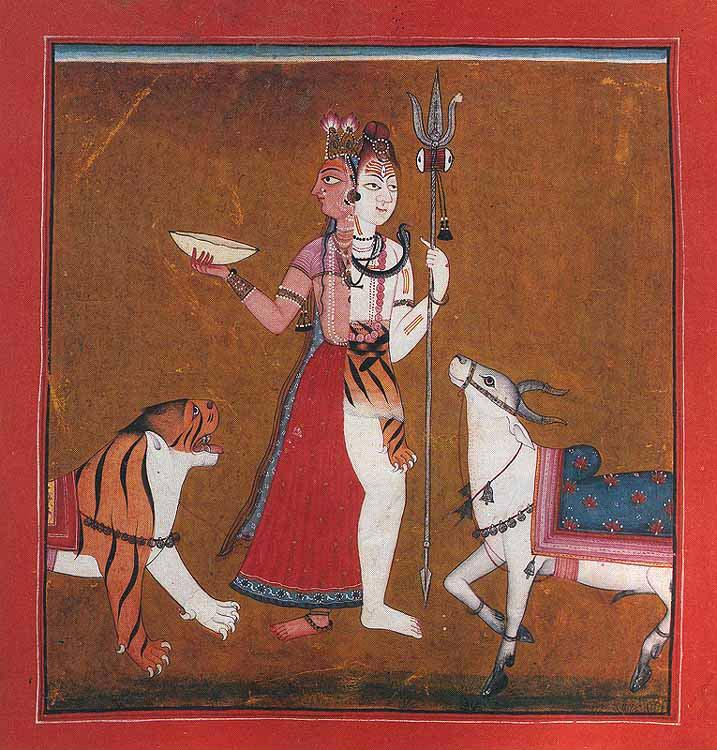
\includegraphics[width=\textwidth]{androgyne.jpg}

Although not mentioned in any of the texts and the word {\em ubhatob­yañ­janaka} does not appear in any texts outside the Buddhist Vinaya and commentaries thereof\footnote{\ref{appendix 2}, \ref{sanskrit1} shows that the {\em ubhatob­yañ­janaka} does not appear in any Vedic or Brahmanical texts and only appears in the Buddhist texts. There is however another word in the {\m Varṣāvastu}, namely {\em strīpuruṣapaṇḍakam} which literally means a {\em paṇḍaka} who is both female and male.}, it seems logical that by the sheer definition of the {\em napuṃsaka} as 'anything that is not entirely male' the {\em ubhatob­yañ­janaka} also falls under this category. As a subcategory of the {\em napuṃsaka} they would have been seen as hyperlibidinous, which is in later texts explained by the fact that {\em napuṃsaka} have both male and female characteristics. 

But the word 'characteristic' is confusing here and seems to be used loosely throughout the Vinaya and commentarial texts. As several authors have pointed out\footnote{\cite{jackson}, quoting Bunmi Methangkun (1986) (article in Thai), observes that psychological as well as physiological factors are involved in the constitution of the {\em ubhatob­yañ­janaka}. He also observes (without reference) that in early Buddhist communities men who engage in receptive anal sex are seen as feminized and thought to be hermaphrodites. See also \cite{zwilling}} and as we have seen in the discussion on Brahmanical and Jain texts, the male and female characteristics are more than merely genital or procreative. It also involves secondary sexual characteristics like the growth of breasts and hair, as well as socio-cultural and psychological characteristics and feelings. That this is equally true for the Buddhist perspective, at least in the (4–5th century CE), is detailed in the Abhidharma Kośa (IV.14c) which approximates that of the Brahmanical view that sex ({\em vyañjana}) is distinguished on the basis of primary and secondary sexual characteristics.

The {\em paṇḍaka} as a subset of {\em napuṃsaka} was also seen as having both male and female characteristics in the Jain scriptures but is obviously not the same as a {\em ubhatob­yañ­janaka}. The difference between the {\em paṇḍaka} and the {\em ubhatob­yañ­janaka} clearly seems to be on the procreative level in that the {\em ubhatob­yañ­janaka} is able to conceive and impregnate while the {\em paṇḍaka}, as an impotent man, can do neither. However, from the descriptions given in the {\em Samantapāsādikā}, the {\em ubhatob­yañ­janaka} is also able to change their secondary characteristics as well as outside appearance and behaviour to appear either male or female. Again, this is not humanly possible outside the realm of mythology.

All the Vinayas agree that the {\em ubhatob­yañ­janaka}/二根 is one of the four sex/gender types next to male, female and {\em paṇḍaka}/黃門. Considering that the male and female were seen as both having just one root/faculty (in the meaning of procreative ability), and the {\em paṇḍaka} has none\footnote{Note that when the {\em paṇḍaka} appears in the texts in the list of these four sex/gender types, it is in the Chinese Vinayas always described with the characters 黃門 ('eunuch') and never as 種不能男 ('impotent'). Indeed we find in the Chinese texts that a eunuch is somebody with the 'male faculty' removed. There might be some confusion here as to what entails characteristics and the Chinese scribes would have only been able to describe this based on their own experiences in their own culture.}, the two-faculties person fills a gap. This could indicate a philosophical position using the {\em catuskoti}\footnote{Dr. M. Vermeulen, book on this subject is yet to be published}. 

Just like the {\em paṇḍaka}, I believe that the {\em ubhatob­yañ­janaka} is a later addition to the Vinaya. The word does not appear in the early suttas\footnote{See \ref{appendix2}, \ref{pali1}} and only briefly in the Vinaya. The description is so brief and hardly existent in the Chinese texts that it seems to be added almost as an after-thought. The insertion would have most likely occurred during the redaction of the Vinaya at the Second Council.

\subsection{Meaning}
The {\em ubhatob­yañ­janaka} seems to be a rather elusive term that does not allow itself to be captured easily. Various scholars have tried to explain this as a form of intersex\footnote{For a brief description of the term 'intersex' see \ref{appendix1}, \ref{intersex}} for the sole reason that intersex people were previously erroneously called 'hermaphrodite' and a hermaphrodite can procreate in both the male and female way as is the exact description of the {\em ubhatob­yañ­janaka} in the commentaries. This is confusing as a true hermaphrodite does not exist among humans and is distinct from intersex. 

From the descriptions in the commentaries, the {\em ubhatob­yañ­janaka} is indeed a true hermaphrodite and therefore not human in nature. It is a mythological or heavenly being, sprung from the same root as the Vedic myths that created the hijra. As \cite{goldman} points out: "... the whole phenomenon appears to be deeply bound up with a patriarchal culture's ambivalent construction of women and their sexuality." The Vedic stories explore the deep longing of men to be able to conceive and the idea found in a variety on Indian sources, including the above mentioned tale of King {\em Bhaṅgāśvana}, that a woman's pleasure in the sexual act is greater than that of a man.

